\title{Integrating Category-Partition Method with Combinatorial Interaction
Testing To Produce T-Way Adequate Test Frames}
\author{Andrew Graff}
\documentclass[a4full,12pt]{article}
%\usepackage{fullpage}
%\usepackage{epsfig}
\usepackage{graphicx}
\graphicspath{ {./images/} }
\begin{document}
\maketitle
\section{Introduction}
Testing is an important step in the process of creating useful software. Who is
  going to use or buy your product if it doesn’t function according to the 
  specifications?  For this reason, there are countless hours dedicated to 
  testing, debugging and maintaining software so that it performs the work 
  expected of it. It can be a challenge to create a sustainable, thorough, and 
  comprehensive test suite that is efficient and effective at testing software.
  
\section{Project Statement}
Category partitioning is a useful method for breaking up a software system to be
  tested, and when combined with TSL, can be useful for generating all possible 
  test cases for the given system partition. Similarly, combinatorial 
  interaction testing is useful for defining a subset of tests that satisfy a 
  T-way pairwise interaction using a model and constraints file. These two 
  methodologies and tools are separate pieces of software that require the user 
  to generate the input to both tools. This project takes on the task of 
  combining these two powerful methods and tools so that the user only needs to 
  generate the category partition test specification, and an adequate coverage 
  set of test frames is generated eliminating the need for the engineer to 
  create the model or constraints for the combinatorial interaction testing.
  
\section{Background}
This project builds on the work of two teams that have come up with solutions to
  two different problems. Here we will explain each of those solutions and the 
  tools created to support them.

The \emph{category-partition method} uses formal test specifications to generate
  test case descriptions. These test case descriptions would then be used to
  create an executable software test. So how do you generate the formal test 
  specifications? Depending on the size of the software system to test, the 
  engineer may need to break the program up into smaller testable blocks. For 
  the purposes of this project, we will use a simple example of a zip command.
  The test specification file can be seen in Fig. \ref{fig:tsl_input}.
\begin{figure}[-htb]
\centering
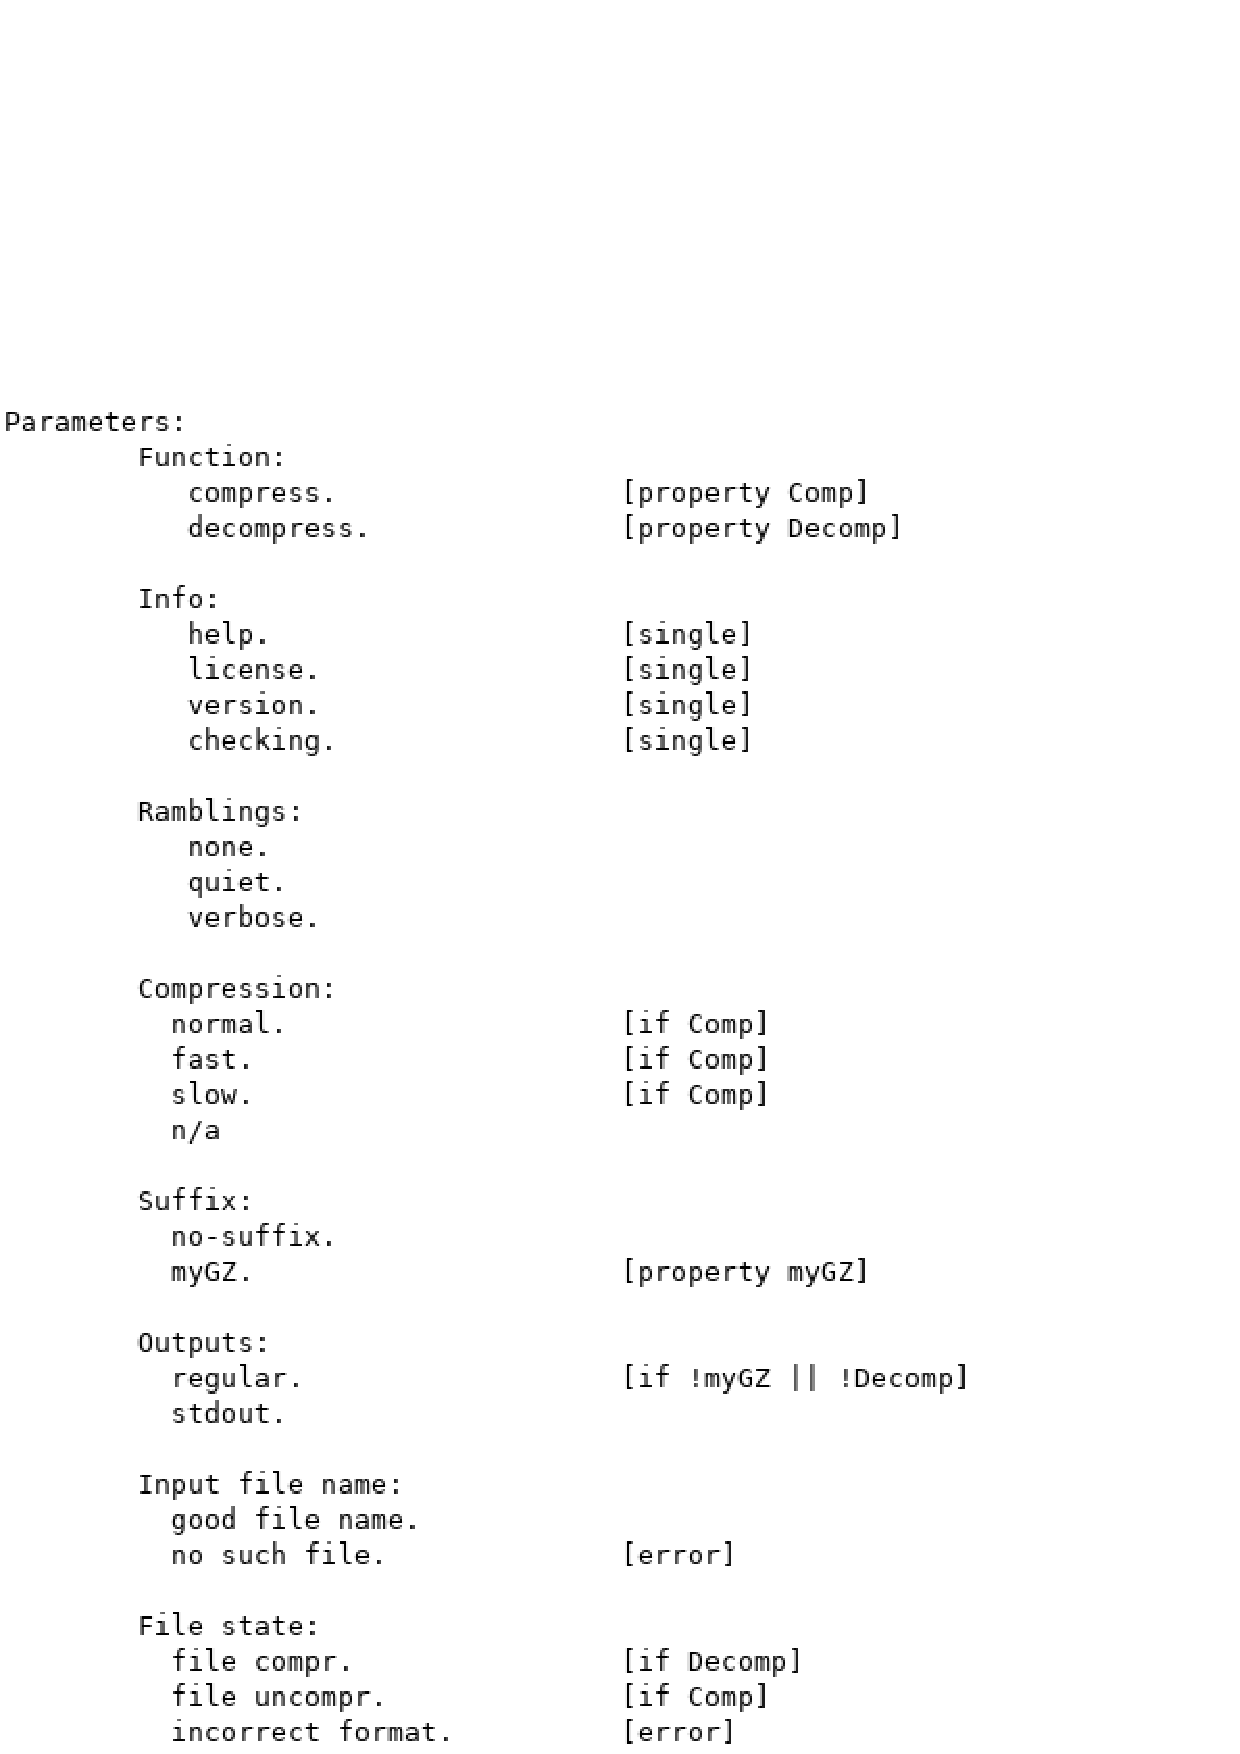
\includegraphics[width=3in,keepaspectratio]{tsl_input.png}
\caption{Category partition input format}
\label{fig:tsl_input}
\end{figure}



Combinatorial Interaction Testing -

\section{Preliminary Work}
Some preliminary work has been done on this project in order to determine if
  the work is sufficient for submission. One of the goals of the project is to
  combine the \emph{tsl} tool with the \emph{casa} tool. Source code was
  acquired for both tools and some initial study of the code was done. As it
  turns out, the \emph{tsl} tool is written in basic C. \emph{casa} on the other
  hand is written in C++. Converting \emph{tsl} to C++ would be beneficial if
  code is to be combined, so that tool has been updated to compile with the g++
  compiler.
  
Another goal of this project is to require the user to only generate the
  category partition test specifications, and the adequate coverage set of test
  frames should be generated. Excluding the contraints file that would be used 
  by \emph{casa} to determine which options can be called with other options, a
  preliminary working version of \emph{tsl} was coded to output the 
  combinatorial interaction testing model required to generate a set the set of
  test frames that would be generated with no contraints. In order to achieve
  this, a new struct was added to \emph{tsl/structs.h} called \emph{container} that
  keeps track of the list of non-single Choices as a vector of Choice struct
  pointers. This vector is used to lookup the choices and categories later for
  printing the test frames. In addition, a \emph{parent} pointer was added to
  the Choice struct so that the Category information can be referenced when
  performing the lookup into the Choice* vector.
  
Rather than output directly all possible test frames, a new function called
  \emph{make\_citmodel()} was written in \emph{tsl/output.c} to write a 
  \emph{.citmodel} file used as an input to \emph{casa}. The function
  \emph{generator(Flag flags)} was also modified to call \emph{make\_citmodel()},
  and then make a system call to casa passing in the \emph{.citmodel} file for
  the input. Then, another function created function called
  \emph{process\_output\_file(string filename)} processes the file output by
  \emph{casa} to generate the test frame final output. Ideally there should be
  no file io required, but this is a rough draft of the final solution.
  
Arguably the bulk of the work will be to translate the \emph{properties} and 
  \emph{contraints} defined in the category parition test specifications into
  the contraints file required by \emph{casa} to properly generate the adequate
  set of test frames rather than all possible combinations.

\end{document}
